\newgeometry{left=25mm,right=25mm,top=15mm,bottom=15mm}
\pagestyle{empty}
\addpart{Beilage}
\section*{Sportbefreiung}
Sehr geehrte Lehrkraft \underline{\hspace{3.5cm}},\\[0.5cm]
hiermit befreie ich mein Kind \underline{\hspace{5cm}} als Mitglied der Dabendorf Orthodoxen Religion aus Glaubensgründen für das folgende Quartal vollständig aus dem Sportunterricht. Der allmächtige Imperator \textit{N} möchte nicht, dass weitere Kinder an den skandalösen Taten des Sportfachbereichs zugrunde gehen. Stattdessen regen wir an, den Sportunterricht mit intellektuell anspruchsvollen Tätigkeiten wie Schach oder Programmieren zu ersetzen. Wir sind uns sicher, dass Ihnen etwas einfallen wird.\\[0.5cm]
Mit gigafabulösen Grüßen und dem Segen des \textit{N}\\
\underline{\hspace{5cm}}, im Namen der DOR\\[1pt]

\noindent\Rightscissors\xdotfill{1pt}[black]

\section*{Prokrastinationszertifikat}
Sehr geehrte Bourgeoisie,\\[0.5cm]
hiermit bestätige ich, dass mein*e Mandant*ööse \underline{\hspace{5cm}} an der chronischen Nervenkrankheit \textit{Prokrastination} leidet, die selbige*n daran hindert, so produktiv zu sein, wie Sie sich das möglicherweise vorstellen. Anzeichen dieses Leidens sind Demotivation und das krampfhafte Suchen nach Alternativbeschäftigung. Es sollte Ihnen bekannt sein, dass das Dabendorfer Rechtsblatt die Opfer dieser Krankheit umfassend schützt. Es sei Ihnen also bewusst, dass Sie verpflichtet sind, \underline{\hspace{5.5cm}} bei vollem Gehalt bis zur Rente weiter zu beschäftigen.\\[0.5cm]
Mit knorkulösen Grüßen und dem Segen des \textit{N}\\
\underline{\hspace{5cm}}\\
Arzt des Dabendorfer Instituts für Prokrastinationsforschung\\[1pt]

\noindent\Rightscissors\xdotfill{1pt}[black]
\section*{Einhornbanner}
\begin{center}

\includegraphics[width=1\textwidth]{bilder/doreinhornBanner}
\end{center}

\clearpage
\section*{Bastelanleitung für Dein eigenes \textit{N}}
\textit{N} ist kein fanatischer Verfechter der Theorie, dass Abbildungen von ihm verboten sein sollten. Ein jeder \textit{Bürger Dabendorfs} ist berechtigt, den Namen des \textit{N} zu verwenden und in Wort und Schrift zu verbreiten, was sogar Franzaken oft unbewusst tätigen. Jeder Gläubige ist zudem aufgerufen, sich den \textit{Quellcode der Klasse N} zu importieren und eine \textit{eigene Instanz von N} zu erzeugen. Die Klasse \textit{N} ist \textit{final}, das heißt sie ist nicht für andere Klassen vererbbar, um die \textit{Einzigartigkeit} des großen \textit{N} zu wahren. Der folgende Codeauszug ist ein Beispiel für \textit{Java}, welcher jedoch weniger als ein Millionstel der vielfältig brillanten Methoden des \textit{N} offenbart.
\lstinputlisting[language=Java,caption=]{bilder/N.java}

\clearpage
\vspace*{\fill}
\begin{center}
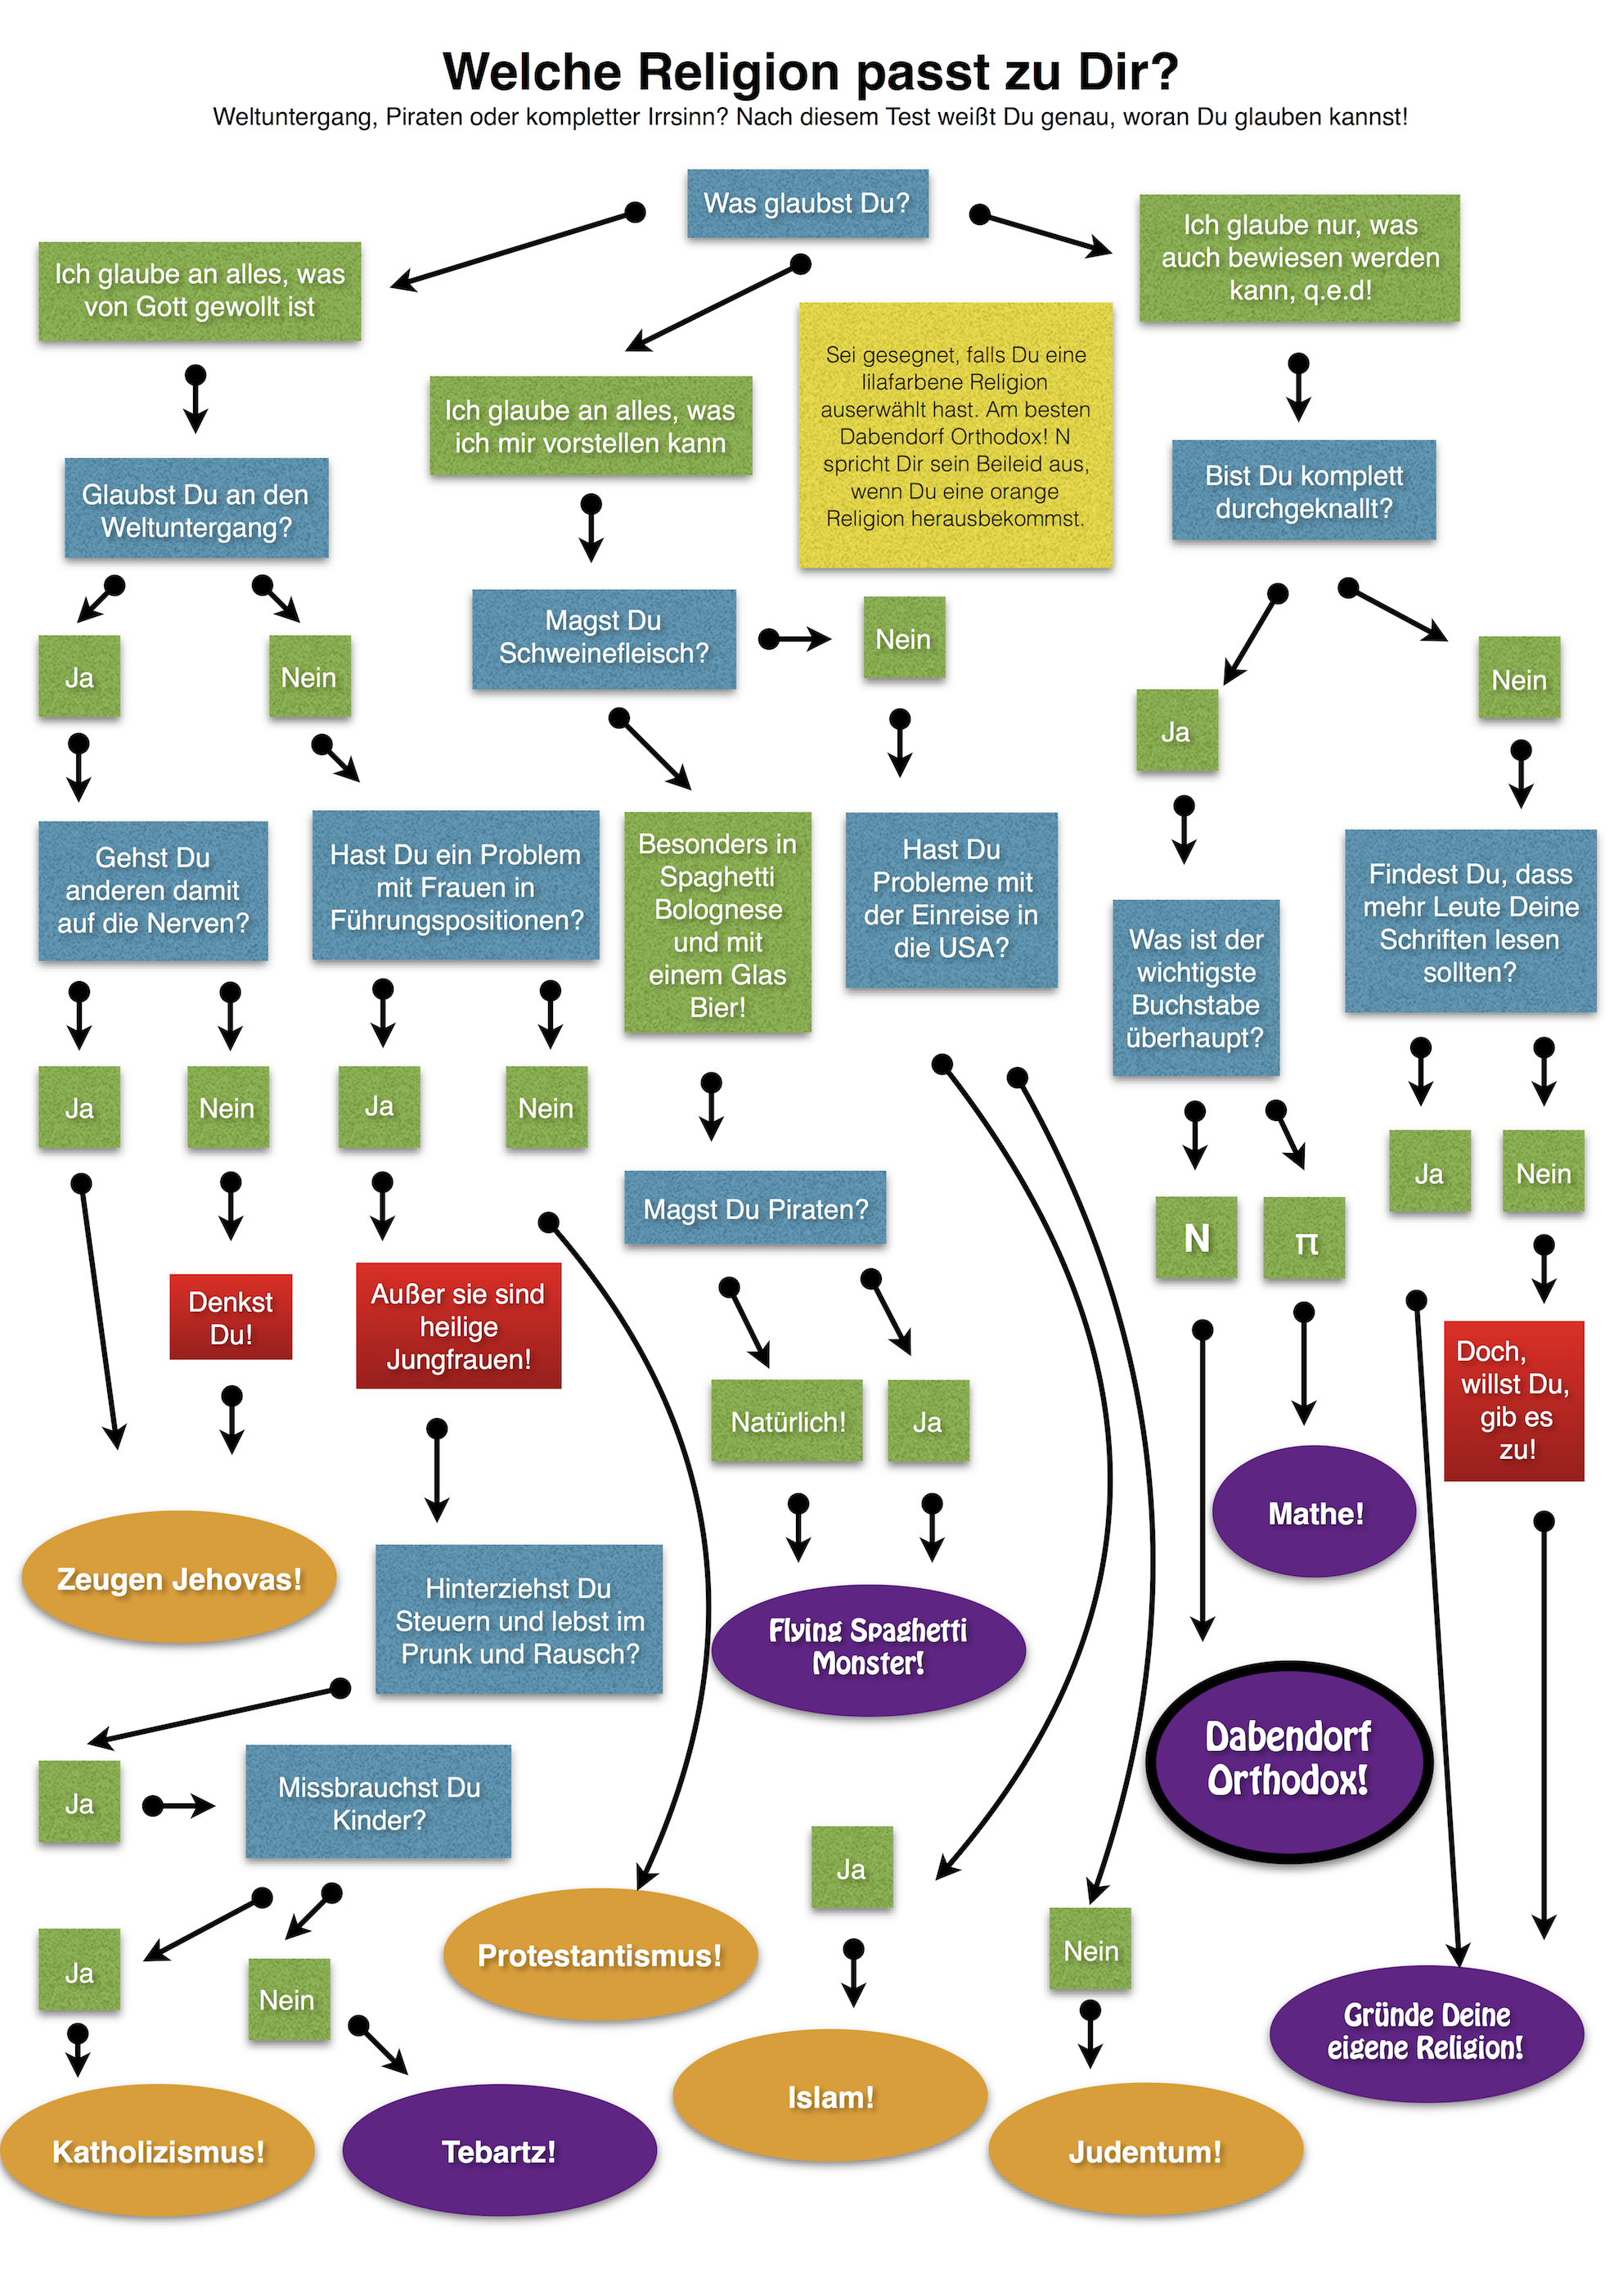
\includegraphics[width=1\textwidth]{bilder/Anhang_Religionsfrage}
\end{center}
\vspace*{\fill}

%Wie viel N
%Kreuzworträtsel?